\begin{comment}
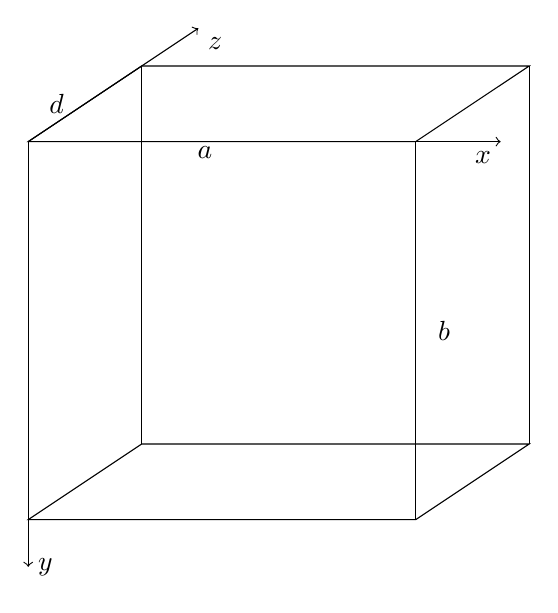
\begin{tikzpicture}[scale=1.2,
    x={(1cm,0cm)},
    y={(0.6cm,0.4cm)},
    z={(0cm,1cm)}
]

    % Parametri
    \def\a{4.1}
    \def\b{4}
    \def\d{2}

    % Assi cartesiani
    \draw[->] (0,0,0) -- (5,0,0) node[below left] {$x$};
    \draw[->] (0,0,0) -- (0,3,0) node[below right] {$z$};
    \draw[->] (0,0,0) -- (0,0,-4.5) node[right] {$y$};

    % Vertici del parallelepipedo
    \coordinate (O) at (0,0,0);
    \coordinate (A) at (\a,0,0);
    \coordinate (B) at (\a,\d,0);
    \coordinate (C) at (0,\d,0);

    \coordinate (O1) at (0,0,-\b);
    \coordinate (A1) at (\a,0,-\b);
    \coordinate (B1) at (\a,\d,-\b);
    \coordinate (C1) at (0,\d,-\b);

    % Spigoli base
    \draw (O) -- (A) -- (B) -- (C) -- cycle;

    % Spigoli verticali
    \draw (O) -- (O1);
    \draw (A) -- (A1);
    \draw (B) -- (B1);
    \draw (C) -- (C1);

    % Spigoli superiori
    \draw (O1) -- (A1) -- (B1) -- (C1) -- cycle;

    % Etichette dimensioni
    \node at (\a/2, -0.3, 0) {$a$};
    \node at (\a+0.3,0,-\b/2) {$b$};
    \node at (-0.3,\d/2,0) {$d$};


    \end{tikzpicture}

\end{comment}
\begin{figure}
    \center
    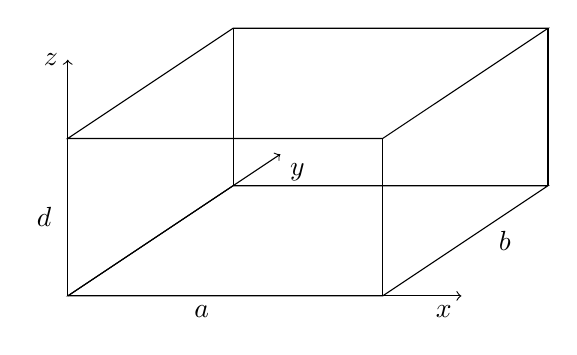
\begin{tikzpicture}[ % FISSA IL RIFERIMENTO IN MODO CORRETTO, ALTRIMENTRI --> (X,Z,Y)
        x={(1cm,0cm)},
        y={(0.6cm,0.4cm)},
        z={(0cm,1cm)}
        ]
            % Parametri
        \def\a{4}
        \def\b{3.5}
        \def\d{2}

        % Assi cartesiani
        \draw[->] (0,0,0) -- ({\a + 1},0,0) node[below left] {$x$};
        \draw[->] (0,0,0) -- (0,{\b + 1},0) node[below right] {$y$}; % below/above
        \draw[->] (0,0,0) -- (0,0,{\d + 1}) node[left] {$z$};

        % Vertici del parallelepipedo
        \coordinate (O) at (0,0,0);
        \coordinate (A) at (\a,0,0);
        \coordinate (B) at (\a,\b,0);
        \coordinate (C) at (0,\b,0);

        \coordinate (O1) at (0,0,\d);
        \coordinate (A1) at (\a,0,\d);
        \coordinate (B1) at (\a,\b,\d);
        \coordinate (C1) at (0,\b,\d);

        % Spigoli base
        \draw (O) -- (A) -- (B) -- (C) -- cycle;

        % Spigoli verticali
        \draw (O) -- (O1);
        \draw (A) -- (A1);
        \draw (B) -- (B1);
        \draw (C) -- (C1);

        % Spigoli superiori
        \draw (O1) -- (A1) -- (B1) -- (C1) -- cycle;

        % Etichette dimensioni
        \node at (\a/2, -0.5, 0) {$a$};
        \node at (\a+0.5, \b/2, 0) {$b$};
        \node at (-0.3, 0, \d/2) {$d$};

    \end{tikzpicture}
    \caption{Cavità a forma di parallelepipedo}
    \label{figure:_cavità_parallelepipedo}
\end{figure}